\documentclass{article}

%other packages
\usepackage[a4paper]{geometry}
\usepackage{longtable}
\usepackage{wrapfig}
\setlength\parindent{0pt}
\usepackage{enumitem}
\usepackage[table,dvipsnames]{xcolor}
\usepackage{polynom}
\def\scaleint#1{\vcenter{\hbox{\scaleto[3ex]{\displaystyle\int}{#1}}}}
\usepackage{array}
\newcolumntype{C}{>{{}}c<{{}}} % for '+' and '-' symbols
\newcolumntype{R}{>{\displaystyle}r} % automatic display-style math mode 
\usepackage{tabularray}
\usepackage{dcolumn,tabularx,booktabs}
\usepackage[most]{tcolorbox}
%\graphicspath{ {C:/Users/twill/OneDrive/Desktop/Eliason/Diagrams} }

%maths
\usepackage{mathtools}
\usepackage{amsmath}
\usepackage{amssymb}
\usepackage{amsfonts}
\usepackage{autobreak}

%tikzpicture
\usepackage{tikz}
\usepackage{scalerel}
\usepackage{pict2e}
\usepackage{tkz-euclide}
\usepackage{tikz-3dplot}
\usetikzlibrary{calc}
\usetikzlibrary{patterns,arrows.meta}
\usetikzlibrary{shadows}
\usetikzlibrary{external}
\usetikzlibrary{decorations.pathreplacing,angles,quotes}

%pgfplots
\usepackage{pgfplots}
\pgfplotsset{compat=1.18}
\usepgfplotslibrary{statistics}
\usepgfplotslibrary{fillbetween}

\pgfplotsset{
    standard/.style={
    axis line style = thick,
    trig format=deg,
    enlargelimits,
    axis x line=middle,
    axis y line=middle,
    enlarge x limits=0.15,
    enlarge y limits=0.15,
    every axis x label/.style={at={(current axis.right of origin)},anchor=north west},
    every axis y label/.style={at={(current axis.above origin)},anchor=south east}
    }
}

\begin{document}

Math 115, 22 March 2024
\hrule

\vspace{10pt}

For questions about areas between curves, Our Math Professor will require that we calculate the points of intersection. A useful visualization trick for integrating with repsect to $y$ is to switch $x$ and $y$, then integrate with respect to $x$. Basically, just redraw the graph, but flipped about $y=x$.

\vspace{10pt}
%https://tex.stackexchange.com/questions/229518/fill-intersection-between-two-parametric-paths-e-g-circles-in-pgfplots
\begin{center}
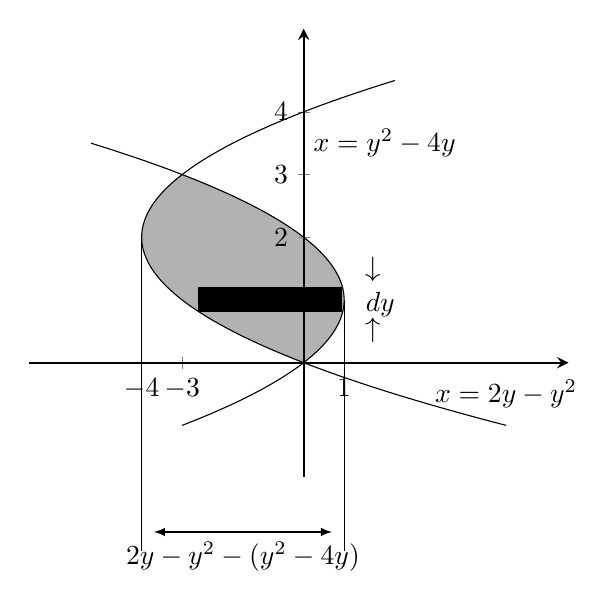
\begin{tikzpicture}
\pgfdeclarelayer{pre main}
    \pgfsetlayers{pre main,main}
\begin{axis}[clip=false,standard,samples=100,xtick={-4,-3,1},ytick={2,3,4}]
\addplot[domain=-1:4.5,name path=F] ({x^2-4*x}, {x});
\addplot[domain=-1:3.5,name path=G] ({-x^2+2*x}, {x});
\begin{pgfonlayer}{pre main}
        \fill [black,opacity=0.3,
          intersection segments={
            of=F and G,
            sequence={R2--L2--R2}
          }];
      \end{pgfonlayer}
\fill[] (0.95,0.8) -- (-2.6,0.8) -- (-2.6,1.2) -- (0.95,1.2) -- node[pos=0.5,right=5pt]{\rotatebox{-90}{$\rightarrow$ \rotatebox{90}{$dy$}$\leftarrow$}} cycle;
\node at (2,3.5) {$x=y^2-4y$};
\node at (5,-0.5) {$x=2y-y^2$};
\draw[] (-4,2) -- (-4,-3);
\draw[] (1,1) -- (1,-3);
\draw[latex-latex] (-3.7,-2.7) -- (0.7,-2.7) node[pos=0.5,below]{$2y-y^2-(y^2-4y)$};
\end{axis}
\end{tikzpicture}
\end{center}

For instance, $\int_0^6-(x^2-4x)+2x\ dx$ is the same thing as the area between $2x$ and $(x^2-4x)$ over $[0,6]$.

\vspace{10pt}

We also considered $\int_0^{2\pi}(-\cos x+2)-(\cos x)\ dx$:

\begin{center}
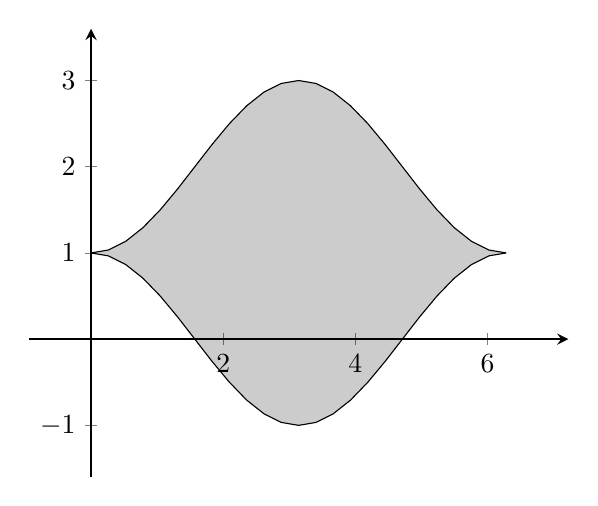
\begin{tikzpicture}
\begin{axis}[standard,domain=0:2*pi]

\addplot[name path=F] {-cos(deg(x))+2};
\addplot[name path=G] {cos(deg(x))};
\addplot[fill=black, fill opacity=0.2] fill between [of=F and G, soft clip={domain=0:2*pi}];
\end{axis}
\end{tikzpicture}
\end{center}

The last question we looked at is a bit worrying, because it requires that you thoroughly understand trigonometric substitution. Specifically, we looked at the area under a line and above a circle, which means subtracting the area of the circle from the area under the line. To calculate the area of the circle, we need to use trig substitution, just as we would use hyperbolic substitution for a hyperbola. It's one thing to look at the fancy formulae, but remembering the shapes andtheir properties goes a long way. It's almost like cheating, visualizing the geometry of the situation in your head.






\end{document}
